\subsection{Verifica della banda passante}
\label{par3:bode}

In questa parte dell'esperienza vogliamo valutare la banda passante di un circuito amplificatore (non invertente) considerando che il guadagno a maglia aperta dell'amplificatore operazionale dipende della frequenza.

\subsubsection*{Funzione di trasferimento e frequenza di taglio}

Esaminiamo dapprima il circuito, calcolandone la funzione di trasferimento. Per ogni amplificatore operazionale vale
\begin{wrapfigure}[20]{l}{0.45\textwidth}
  \begin{center}
    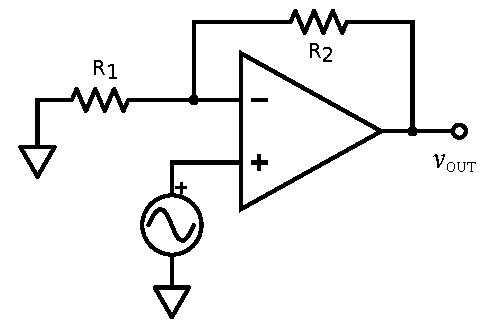
\includegraphics[width=0.32\textwidth]{../E03/latex/bandwidth.pdf}
  \end{center}
  \caption{Schema del circuito utilizzato per valutare la banda passante. La resistenza $R_1=997\pm1$ \si{\ohm} è fissa; mentre $R_2$ è stata cambiata con valori $R_2^{11\mathrm{x}}=9.91 \pm 0.01$ \si{\kilo\ohm} e $R_2^{101\mathrm{x}}=99.1 \pm 0.1$ \si{\kilo\ohm} a seconda del guadagno desiderato.}
  \label{cir3:banda}
\end{wrapfigure}
\begin{equation}
V_{out}=A(s) (V^+-V^-)
\label{eq3:regola_opamp}
\end{equation}
con il guadagno, come detto sopra, che in generale dipende da $s=j\omega$ (e quindi dalla frequenza). Consideriamo
$$V^+ = V_{in} \qquad V^-=V_{out} \frac{R_1}{R_1+R_2}$$
dove $V^-$ è ricavato dalla solita formula per l'amplificatore non invertente $(V^+-V^-)/R_1 + (V_{out}-V^-)/R_2 =0$. Definiamo
$$\beta = \frac{R_1}{R_1+R_2} = \frac{1}{G}$$
Si noti che $G$ è il guadagno circuitale di un amplificatore non invertente. Sostituendo questi valori in (\ref{eq3:regola_opamp}) otteniamo
$$A(s) V_{in} = V_{out} + V_{out} A(s) \beta$$
Calcoliamo ora la funzione di trasferimento $H$
\begin{equation}
H(s)=\frac{V_{out}}{V_{in}}=\frac{1}{\beta}\frac{1}{1+\frac{1}{A(s) \beta}}
\label{eq3:funz_trasfe}
\end{equation}
da cui è facile notare che per $A(s) \rightarrow + \infty$ (approssimazione di amplificatore ideale), $H(s)=\frac{1}{\beta}=1+\frac{R_2}{R_1}=G$, equazione che diventa indipendente dal guadagno a maglia aperta.

Schematizziamo l'OPAMP come un filtro passa basso. Abbiamo che il guadagno a maglia aperta varia con la frequenza secondo la legge
$$A(j\omega)=\frac{A_{ol}}{1+j\frac{\omega}{\omega_0}}$$
con $\omega_0 \approx 8$ \si{\hertz} la prima frequenza di taglio dell'operazionale data dalla capacità di compensazione nella circuiteria interna e $A_{ol}$ il guadagno dell'operazionale con segnali costanti ($f = 0$). Sostituendo questo valore in (\ref{eq3:funz_trasfe}), abbiamo
\begin{equation}
H(j\omega)=\frac{\frac{A_{ol}}{1+A_{ol}\beta}}{1+j \frac{\omega}{(1+A_{ol}\beta)\omega_0}}
\label{eq3:funzione_trasferimento}
\end{equation}
da cui si nota che la nuova frequenza di taglio è data da
\begin{equation}
\omega_t=(1+A_{ol}\beta)\omega_0
\label{eq3:freq_taglio}
\end{equation}
Nel circuito in Figura \ref{cir3:banda} avevamo un guadagno $G$ retroazionato di $11$ e $101$, quindi ci aspettiamo\footnote{Questi valori sono approssimati perchè cercheremo di calcolare $A_{ol}$ con le frequenze a nostra disposizione, ricavate con l'analisi della banda, piuttosto che calcolare ora frequenze di taglio senza essere certi del valore di $A_{ol}$.} frequenze di taglio, per l'equazione precedente, rispettivamente sull'ordine dei $10^5$ e $10^4$. Per fare una stima delle frequenze di taglio era anche possibile sfruttare la costante \textit{gain-bandwidth product} GBWP $= 2 \pi \omega_t G$, costante dell'amplificatore operazionale.

\subsubsection*{Effetto dello Slew Rate}

Ovviamente, durante la misurazione bisogna minimizzare l'effetto dello Slew Rate che, come visto nel paragrafo precedente, distorce la forma d'onda in uscita. Bisogna quindi scegliere valori di tensione del segnale in ingresso appropriati.
Supponiamo dunque di avere una forma d'onda in uscita del tipo $V_{out} \sin (2 \pi f_0 t) = V_{in} G \sin (2 \pi f_0 t)$. Vale, affinché non si raggiunga lo SR
$$\mathrm{max}\left[ \frac{dV_{out}}{dt} \right] = \mathrm{max} \left[ 2 \pi V_{in} G f_0 \cos (2 \pi f_0 t) \right]= 2 \pi V_{in} G f_0 < 0.35 \si{\volt\per\micro\second}$$
dove l'ultimo valore è stato scelto per tenerci sempre abbastanza distanti dal valore reale di SR. Dunque vale che
\begin{equation}
V_{in}<\frac{0.35 \si{\volt\per\micro\second}}{2 \pi G f_0} = \frac{0.35 \si{\volt\per\micro\second}}{2 \pi \mathrm{GBWP}}
\label{eq3:tensione_max}
\end{equation}
Considerando $f_0$ come la frequenza di taglio stimata prima, otteniamo che i valori di tensione da usare nei due casi è di circa $V_{in}^{11\mathrm{x}} = 100$ \si{\milli\volt}$= V_{in}^{101\mathrm{x}}$. Si nota che la regola \ref{eq3:tensione_max} è valida quando il guadagno non dipende dalla frequenza: infatti dopo la frequenza di taglio il guadagno del circuito $G$ cala e dunque i valori di tensione ammessi risultano di valore maggiore.

\subsubsection*{Grafici di Bode}

\begin{figure}[ht]
 \centering
   {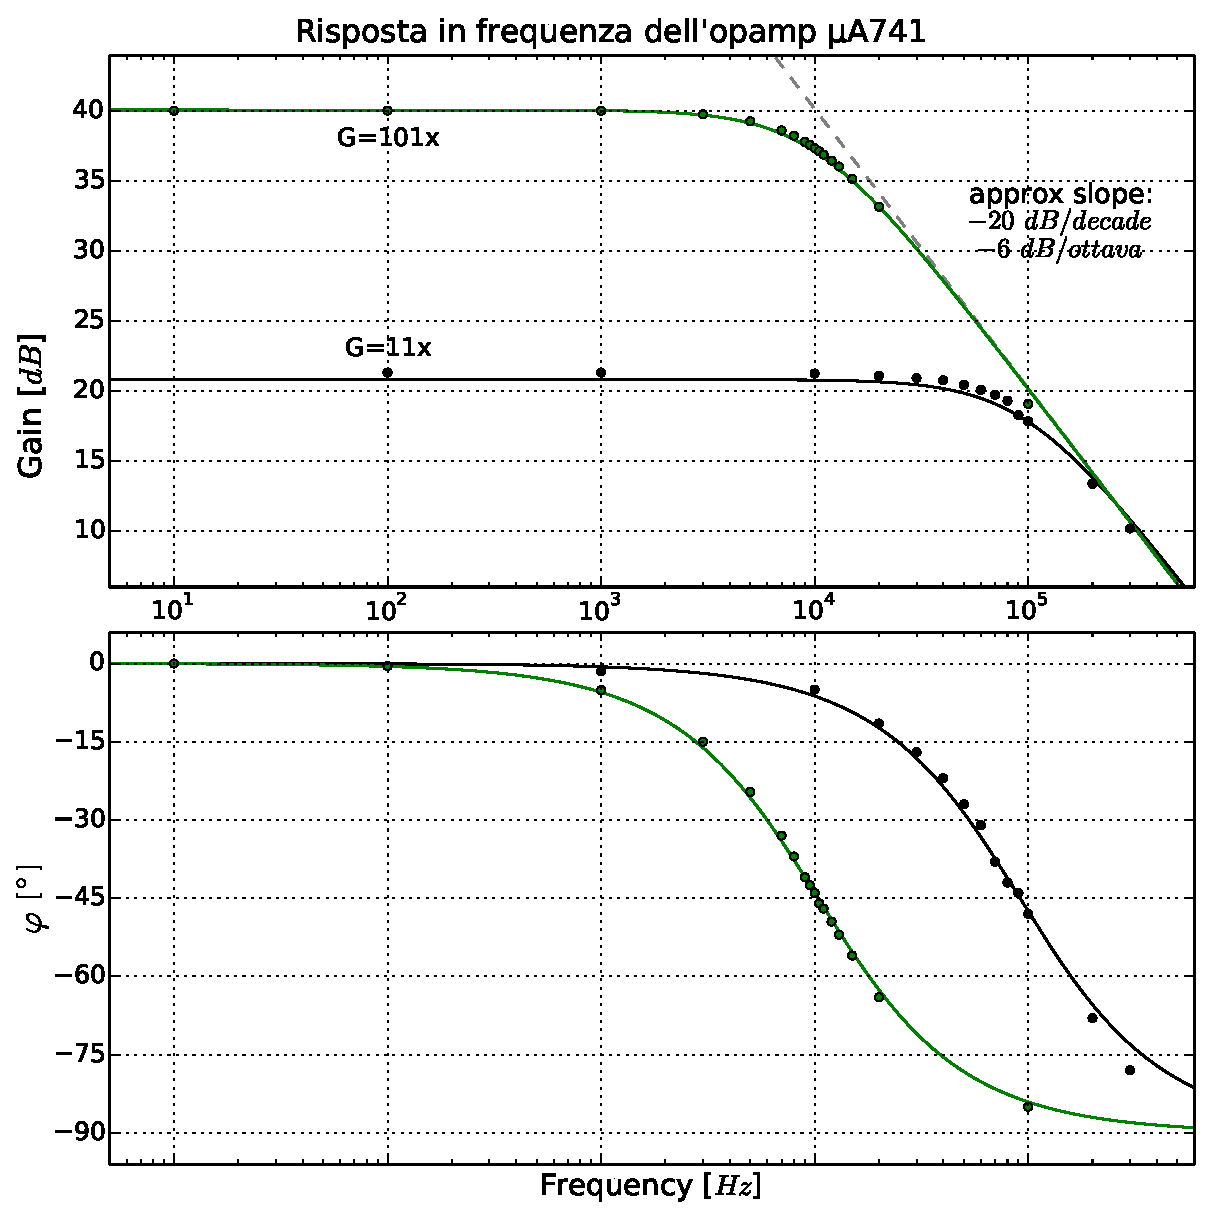
\includegraphics[width=0.75\textwidth]{../E03/latex/bode.pdf}}
 \caption{Diagrammi di Bode per il guadagno del circuito in Figura \ref{cir3:banda}.}
 \label{gr3:bode}
\end{figure}

Utilizzando una forma d'onda sinusoidale abbiamo dunque misurato la tensione di uscita del circuito e la fase fra i segnali, per poi plottare i grafici di Bode (Figura \ref{gr3:bode}).

Dalla funzione di trasferimento (\ref{eq3:funzione_trasferimento}) possiamo inoltre trovare le relazioni fra il guadagno e la fase con la frequenza. Sappiamo infatti che il guadagno è dato $V_{out}/V_{in}$, ed in generale queste due tensioni possono essere considerate come complesse. Se siamo dunque interessati al guadagno dobbiamo considerare piuttosto il rapporto dei moduli, ed otteniamo la seguente relazione
\begin{equation}
\mathrm{Gain}=\frac{|V_{out}|}{|V_{in}|}=|H(j\omega)|=\sqrt{\frac{A_{ol}^2 \omega_0^2}{(\omega_0 + A_{ol} G \omega_0)^2 + \omega^2}}
\label{eq3:fit_gain}
\end{equation}
mentre, per la fase utilizziamo la solita formula della fase per un numero complesso (nel nostro caso $V_{out}/V_{in}$), ed otteniamo
\begin{equation}
\varphi=\arctan\left[{\frac{\mathrm{Im}[H(j\omega)]}{\mathrm{Re}[H(j\omega)]}}\right]= - \arctan\left[\frac{\omega}{(1+A_{ol}G)\omega_0}\right]
\label{eq3:fit_fase}
\end{equation}

Date queste leggi è possibile stimare $A_{ol}$ e $\omega_0$ dell'operazionale: rimandiamo al paragrafo \ref{par3:A_ol} per questi calcoli, dove saranno confrontati i valori ottenuti con questi dati e quelli presi al paragrafo \ref{par3:open}.

Infine, i valori di frequenza di taglio possono essere calcolati dalla legge al valore di fase del flesso ($45^{\circ}$). Questi sono: $f_t^{101\mathrm{x}} = (10.3 \pm 0.1)$ \si{\kHz} e $f_t^{11\mathrm{x}} = (92 \pm 1)$ \si{\kHz}, in accordo con gli ordini di grandezza stimati in precedenza.